\chapter{Goals and Use Cases}
\label{ch:Goals and Use Cases}

In this chapter, the intended goals of the project and some use cases are being discussed.

\section{Goals}

The goal of the project is to develop a software suite which facilitates interoperability between MANO frameworks, thereby enabling the management of a network service across multi-vendor environments. To achieve this, the software suite is divided into 3 individual work packages (WPs), which are initially developed in parallel and are merged later. In the following sections, the individual goals of these work packages are explained in detail.

\subsection{Service Descriptor Translator (SDT)}

In this work package, a translator engine for a NSD is implemented. The Network Function Virtualization Orchestrator (NFVO) is the main orchestration unit of a MANO framework that manages the lifecycle of a network service. One of the main functions of a NFVO is registering a network service, by onboarding, it's NSD to the network service catalog. In a scenario, where a network service is to be deployed and registered among two different MANO
frameworks, having their own NSD schema respectively, our SDT engine would help in translating a NSD schema from one MANO framework to the other framework. To accomplish this, the NSD schema from the network service catalog of the two different MANO frameworks needs to be extracted and passed on to SDT engine. SDT engine consumes the NSD schemas and translates one NSD schema to the other MANO framework's NSD schema. REST interfaces are made available for other services to interface with the SDT.

\subsection{Service Descriptor Splitter (SDS)}

In the production environment, a network service is deployed over a vast geographical region spanning multiple domains. In such scenarios, there is a need to split a network service into smaller network services and deploy it over multiple domains. In this work package, a Service Descriptor Splitter (SDS) is implemented which splits the NSD of a network service. SDS takes NSD as an input that contains all the information elements which can be extracted to generate separate NSDs. In the proposed approach, the Service Graph is extracted from the input NSD and is split into subgraphs that result in a separate set of elements such as VNFs, virtual links, forwarding graphs of VNFs etc. Different network graph splitting algorithms are then evaluated to split the service graph. These sets are considered to generate NSDs according to the domain-specific orchestrators.


\subsection{MANO Adaptor (MA)}

A key component of a MANO framework is Virtualized Interface Manager (VIM),  which helps in assigning the hardware resources to virtual resources. The MANO framework uses specific adaptors to communicate with their respective VIMs. For instance, Sonata  (\ref{SecSONATA}) MANO framework has adaptors for OpenStack (\ref{SecOpenStack}) and Kubernetes (\ref{SecKubernetes}). However, when there is a spike in the service request beyond the capabilities of a single MANO instance, multiple MANO instances should be instantiated to balance the load. The goal of this work package is to build an adaptor that facilitates interaction between different instances of MANO frameworks, thereby exposing the underlying MANO framework's interfaces and enabling monitoring of the underlying service states.

Apart from the implementation of MA, the plan to investigate MANO scalability challenges (See \ref{wp3manoresearch})

\begin{figure}[h]
	\centering
	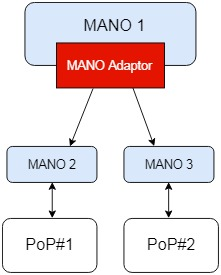
\includegraphics[width=0.29\linewidth]{figures/Structure2}
	\caption{This figure visualizes the structure of MA. }
	\label{fig:structure2}
\end{figure}

\begin{figure}[h]
	\centering
	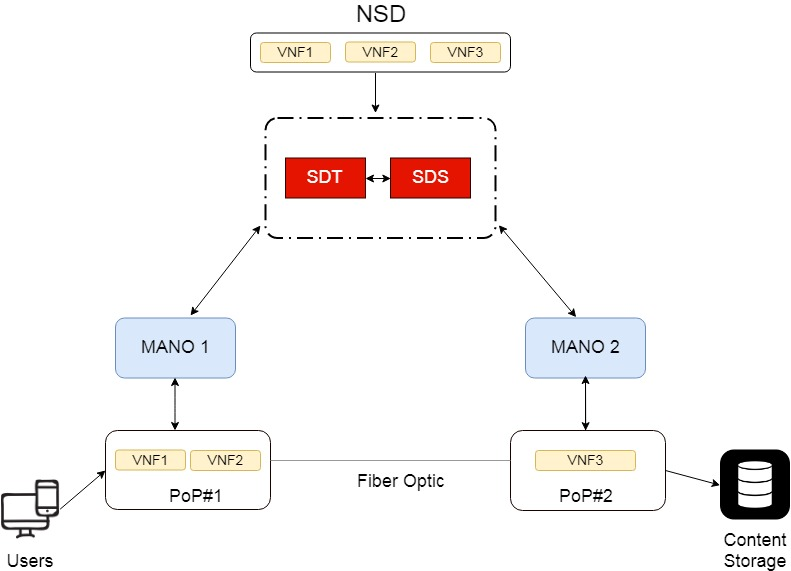
\includegraphics[width=0.7\linewidth]{figures/Structure1}
	\caption{This figure visualizes the structure of SDT and SDS. }
	\label{fig:structure1}
\end{figure}

\subsection{Integration Of Work Packages}
In this work package, the SDT, SDS, and MA are integrated. This integration will augment the functionality of the MA in terms of addressing the scalability challenges between instances of different MANO frameworks. It also extends the capabilities of both the SDS and SDT to split a NSD and then deploy a part of it to a different MANO framework. All these individual modules are planned to be implemented as microservices and integrated keeping their individual autonomy intact. 


\section{Use Cases}

\subsection{Cross-MANO Framework Interaction}
The MANO frameworks used by every network service provider varies from one another. NSD translation enables the deployment of network services that is in accordance with the intended framework.

For instance: Consider two Network Service Operators using different MANO frameworks. One of them uses Sonata framework \cite{draxler2017sonata} and another operator uses OSM framework \cite{ersue2013etsi}. These frameworks have different NSD schemata(refer \ref{SecSONATA} and \ref{SecOSM}). NSD schemata contain VNFs, virtual links, and VNF forwarding graphs and also describes the deployment of a network service. By using a translator, these NSD schemata can be translated into a framework-specific schema. With this, operators can deploy and manage network services across different MANO implementations.

\subsection{Hierarchical Orchestration}
By using the MANO adapter, dynamic instantiation of multiple MANO instances and inter-operability between different MANO frameworks can be achieved. The operator will be able to handle the resources in an efficient manner, as one MANO framework can manage a limited number of service requests, operators can explore options to include additional MANO instances under the existing MANO instance to mitigate the traffic load on a single instance. The resources can be provisioned based on the number of requests. This helps the operator in extending their profitability.
\newpage
\textbf{Actors} : The Network Service Providers who would use features of SCrAMbLE.

\begin{figure} [h]
	\centering
	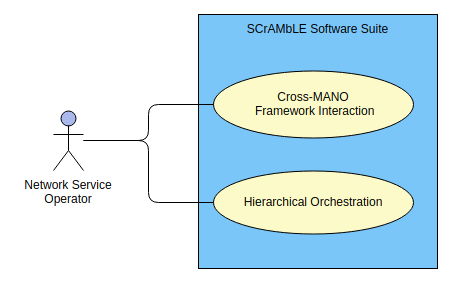
\includegraphics[width=0.9\linewidth]{figures/use-case}
	\caption{Use Case Diagram}
	\label{fig:use-case}
\end{figure}





